\documentclass[11pt]{article}

\usepackage[a4paper,margin=27mm]{geometry}
\usepackage{fontspec}
\usepackage{xeCJK}
\usepackage{unicode-math}
\setmainfont{TeX Gyre Termes}
\setsansfont{TeX Gyre Heros}
\setmonofont{TeX Gyre Cursor}
\setmathfont{TeX Gyre Termes Math}
\setCJKmainfont{Noto Serif CJK SC}
\setCJKsansfont{Noto Sans CJK SC}
\setCJKmonofont{Noto Sans Mono CJK SC}
\usepackage{microtype}
\usepackage{amsthm}
\usepackage{booktabs}
\usepackage{tabularx}
\usepackage{longtable}
\usepackage{array}
\usepackage{enumitem}
\usepackage{graphicx}
\usepackage{tikz}
\usetikzlibrary{arrows.meta,positioning,fit,calc,decorations.pathreplacing}
\usepackage[numbers,sort&compress]{natbib}
\usepackage{xcolor}
\usepackage{seqsplit}
\usepackage{url}
\usepackage{hyperref}
\usepackage[nameinlink,noabbrev]{cleveref}

\hypersetup{
  unicode=true,
  pdftitle={Isotropy Averaging Erases Returns: Character Traces and a Fixed-Map Normality Obstruction on Deninger Prime Orbits},
  pdfauthor={Liang Wang},
  pdfsubject={Transformation groupoids, isotropy characters, and trace normality},
  pdfkeywords={transformation groupoid, isotropy character, Plancherel trace, normal extension, arithmetic dynamics},
  colorlinks=true,
  linkcolor=blue!45!black,
  citecolor=green!35!black,
  urlcolor=blue!55!black
}

\setlength{\parindent}{1.35em}
\setlength{\parskip}{0.25em}
\setlist{nosep,leftmargin=2em}
\setlength{\emergencystretch}{3em}
\renewcommand{\arraystretch}{1.14}
\newcolumntype{Y}{>{\raggedright\arraybackslash}X}
\newcolumntype{P}[1]{>{\raggedright\arraybackslash}p{#1}}

\newtheorem{theorem}{Theorem}[section]
\newtheorem{proposition}[theorem]{Proposition}
\newtheorem{lemma}[theorem]{Lemma}
\newtheorem{corollary}[theorem]{Corollary}
\theoremstyle{definition}
\newtheorem{definition}[theorem]{Definition}
\newtheorem{remark}[theorem]{Remark}

\newcommand{\R}{\mathbb{R}}
\newcommand{\C}{\mathbb{C}}
\newcommand{\Z}{\mathbb{Z}}
\newcommand{\T}{\mathbb{T}}
\newcommand{\K}{\mathcal{K}}
\newcommand{\B}{\mathcal{B}}
\newcommand{\dd}{\,\mathrm{d}}
\newcommand{\e}{\mathrm{e}}
\newcommand{\ii}{\mathrm{i}}
\newcommand{\Tr}{\operatorname{Tr}}
\newcommand{\Tau}{\mathrm{T}}
\newcommand{\supp}{\operatorname{supp}}
\newcommand{\NOTTESTABLE}{\textsc{not\_testable}}
\newcommand{\REFUTED}{\textsc{refuted}}
\newcommand{\PASS}{\textsc{pass}}
\newcommand{\RouteA}{\textsc{Route A}}
\newcommand{\cand}[1]{\nolinkurl{#1}}
\newcommand{\coord}[1]{\texttt{\detokenize{#1}}}

\title{\textbf{Isotropy Averaging Erases Returns: Character Traces and a Fixed-Map Normality Obstruction on Deninger Prime Orbits}}
\author{Liang Wang\\
\small School of Artificial Intelligence and Automation\\
\small Huazhong University of Science and Technology (HUST)\\
\small \href{mailto:wangliang.f@gmail.com}{wangliang.f@gmail.com}}
\date{14 August 2026}

\begin{document}
\maketitle

\begin{abstract}
For an actual periodic orbit already chosen inside Deninger's finite-kernel prime packet, with primitive period \(L=\log p\), we construct the continuous transformation groupoid and identify its full and reduced \(C^*\)-algebras with the same unstabilized algebra \(C(\T)\otimes\K(L^2[0,L))\).  The isotropy character \(\chi_\theta(rL)=\e^{\ii r\theta}\) produces Floquet frequencies \((2\pi n-\theta)/L\) and the trace formula
\[
 \tau_\theta(a_f)=L\sum_{r\in\Z}f(rL)\e^{\ii r\theta},
 \qquad f\in C_c^\infty(\R).
\]
In contrast, the Zak-decomposed source-fibre regular representation has bicommutant \(L^\infty(\T,\dd\theta/(2\pi))\bar\otimes\B(L^2[0,L))\), and its faithful normal semifinite trace is \(\Tau_L(a_f)=Lf(0)\): dual-Haar averaging erases every nonzero return.  Each \(\tau_\theta\) is a lower-semicontinuous, densely defined, semifinite, nonfaithful, unbounded \(C^*\)-trace, but a full finite rank-one corner proves that it has no normal extended-positive extension along this fixed one-orbit map.  Thus the fixed local analogue is \REFUTED.  The packet-level question remains \NOTTESTABLE, because packet Hausdorff/local-compactness and a same-map packet restriction or disintegration theorem are unavailable.  Separately, closed-point counting gives the positive-time scalar Radon measure \(\Theta_+=\sum_p\log p\sum_{r\geq1}\delta_{r\log p}\), so that typed scalar claim is a \PASS.  Deterministic target-free controls verify signs, scales, finite-corner witnesses, and domain separation, but provide no packet, determinant, or spectral claim.

\medskip
\noindent\textbf{Keywords:} transformation groupoid; isotropy character; Plancherel trace; lower-semicontinuous trace; normal extension; Poisson summation; arithmetic dynamics
\end{abstract}

\begin{center}
\textbf{中文摘要}
\end{center}
本文从 Deninger 有限核素数包中一个已经选定的真实周期轨道出发，并严格保留其本原周期 \(L=\log p\)。轨道作用群胚的满与约化 \(C^*\)-代数相同，且可具体写成未再稳定化的 \(C(\T)\otimes\K(L^2[0,L))\)。各向同性特征 \(\chi_\theta(rL)=\e^{\ii r\theta}\) 导出 Floquet 频率 \((2\pi n-\theta)/L\) 以及带相位的返回梳状迹；平凡特征保留全部双向重复返回。与此相反，同一局部对象的源纤维正则表示经 Zak 分解后，其忠实正规半有限迹仅给出 \(Lf(0)\)，对偶 Haar 平均精确消去所有非零返回。有限满秩一角上的递减尖峰进一步表明，特征迹不能沿这一固定局部映射正规延拓，因此固定单轨道版本的结论为 \REFUTED。由于原始素数包的 Hausdorff/局部紧致性以及包层面的同映射限制或分解桥梁尚未证明，包层面的主要问题仍为 \NOTTESTABLE，而不能由局部反例替代。另一方面，按有理闭点计数所得的正时间标量测度 \(\Theta_+=\sum_p\log p\sum_{r\geq1}\delta_{r\log p}\) 在紧集上局部有限，故这一严格分型的标量结论为 \PASS。文中的无目标控制只检查符号、归一化、角压缩和定义域边界；本文不提出包群胚完成、全素数算子、行列式、解析延拓或 Hilbert--Pólya 型结论。

\medskip
\noindent\textbf{中文关键词：} 变换群胚；各向同性特征；Plancherel 迹；下半连续迹；正规延拓；Poisson 求和；算术动力系统

\tableofcontents

\section{Introduction}

Deninger's rational-Witt construction associates to a rational closed point \((p)\subset\operatorname{Spec}\Z\) a packet of periodic trajectories whose common primitive period is \(\log p\) \cite[Section~6 and Theorem~6.1, arXiv-v4 pp.~38--39]{Deninger2026}; the compact-packet statement is also recorded in \cite[Theorem~4.2, arXiv-v1 pp.~11--12]{Deninger2023}.  This source fact suggests an operator-algebraic question that must be typed carefully: can the packet's common isotropy select a return-sensitive trace that is normal on a source-selected regular completion?  Three logically separate answers emerge.

First, for one actual orbit that has already been chosen, the local operator problem is completely decidable.  The groupoid algebra is \(C(\T)\otimes\K\); integration over the isotropy dual gives a faithful normal semifinite (FNS) trace, while evaluation at one isotropy character gives a lower-semicontinuous \(C^*\)-trace.  The former retains only time zero and the latter retains a phase-weighted return comb.  A full finite corner then proves that the character trace cannot extend normally through the fixed regular representation.  The fixed one-orbit analogue is therefore \REFUTED.

Second, the inherited packet is not interchangeable with one orbit.  Its open-cover compactness and second countability are available, but the Hausdorff and locally compact Hausdorff (LCH) gates needed for the frozen standard groupoid completion are open.  No restriction, compression, or disintegration theorem puts the local corner and a packet trace on one represented map.  Consequently the packet-level question is \NOTTESTABLE, not refuted.  The distinction is mathematical rather than rhetorical: a normal-extension assertion has no truth value until both its domain map and codomain von Neumann algebra have been constructed.

Third, a scalar assembly does not require such a packet completion.  There is one rational closed point \((p)\) for each prime, and its source clock is \(L_p=\log p\).  Counting these closed points once produces a locally finite positive-time Radon measure.  This scalar result is a \PASS, but it is neither a packet trace nor a global all-prime operator.

\subsection{Contributions and verdict hierarchy}

The central contribution is the fixed-map normality obstruction.  Its force comes from comparing two traces on one exact local \(C^*\)-algebra and one exact embedding into a diffuse regular von Neumann algebra.  The calculation also makes a structural loss visible: Plancherel averaging is normal precisely where it integrates over the character circle and annihilates every nonzero Fourier coefficient.  The return-sensitive point fibre avoids that cancellation only by becoming nonnormal relative to the fixed regular completion.

The remaining contributions close the mathematical bookkeeping required to make that statement valid: an actual, unstabilized \(C(\T)\otimes\K\) completion; the sign-locked induced representations; trace-class Poisson summation; the Zak bicommutant and FNS domains; a corrected orbit-versus-packet topology split; a positive-time scalar ledger; and target-free falsification controls.  \Cref{tab:p8} records the adjudicated scope.

\begin{table}[htbp]
\centering\small
\caption{Theorem/status audit for P8-1--P8-9.  A scoped or split entry is not an unqualified pass.}\label{tab:p8}
\begin{tabularx}{\textwidth}{P{0.08\textwidth}P{0.19\textwidth}Y Y}
\toprule
Target & Verdict & Proved content & Mandatory boundary\\
\midrule
P8-1 & split pass / \NOTTESTABLE & Every chosen actual orbit closes; the packet has a free compact action and an open quasi-compact second-countable quotient. & Packet and quotient Hausdorff/LCH gates remain open.\\
P8-2 & closed locally & \(A_L\cong C(\T)\otimes\K(H_0)\) as an actual unstabilized isomorphism. & The trivialization is choice-dependent and one-orbit only.\\
P8-3 & closed locally & Trace-class Floquet fibres with frequency \((2\pi n-\theta)/L\) and phase \(\e^{\ii r\theta}\). & The symbolic proof, not finite controls, owns the sign.\\
P8-4 & closed on fixed map & Zak bicommutant and FNS trace \(\Tau_L(a_f)=Lf(0)\). & Normality and cancellation belong only to the fixed regular owner.\\
P8-5 & closed locally & The l.s.c., densely defined, semifinite, nonfaithful character trace gives the full phase comb. & It is unbounded and not normal in the fixed regular completion.\\
P8-6 & closed on fixed map & A full finite corner gives the no-normal-extension theorem; distinct singular corner-state extensions exist. & No full singular extension of the unbounded trace is constructed.\\
P8-7 & scoped pass & Continuous orbit averaging and local/finite/positive-time scalar ledgers are valid on typed domains. & No packet Radon lift, packet trace, or same-map bridge.\\
P8-8 & pass as controls & Eighteen target-free checks and nine deterministic CSV artifacts pass. & Finite checks are witnesses, not proofs.\\
P8-9 & pass as audit & T0--T7 and Route coordinates are evaluated record by record. & No coordinate may be spliced across owners.\\
\bottomrule
\end{tabularx}
\end{table}

\subsection{Prior mathematics, search boundary, and nonclaims}

The operator-algebraic ingredients are classical.  Green imprimitivity \cite[Proposition~3, p.~203]{Green1978}, transitive-groupoid equivalence \cite[Theorems~2.8 and~3.1, pp.~10 and~16]{MuhlyRenaultWilliams1987}, and the exact homogeneous-space specialization \cite[equation~(4.63) and Theorem~4.30, p.~138]{Williams2007} identify the local algebra.  Stable isomorphism alone would be weaker \cite[Theorem~1.2, pp.~351--352]{BrownGreenRieffel1977}; we do not cancel a stabilization.  Amenability supplies full/reduced equality \cite[Examples~2.7(2) and Theorem~5.3]{AnantharamanDelaroche2002}.  Invariant-measure crossed-product traces, Plancherel weights, lower-semicontinuous traces, Morita induction, and normality criteria are available in \cite{BourneRennie2018,Renault2021,ElliottRobertSantiago2011,CombesZettl1983,Jones2009}.  Our use of Poisson summation follows the Fourier convention of \cite[Definition~14.1 and Theorem~23.5]{Laugesen2017}.

The source-to-operator conjunction is stated only with a dated search boundary.  To our knowledge, based on the arXiv, OpenAlex, Crossref-metadata, publisher/author-page, exact-web, and retained-full-text searches documented through 14 August 2026, we did not locate a primary paper that connects Deninger's rational-Witt finite-kernel prime packets to the continuous-\(\R\) transformation-groupoid \(C^*\)/Plancherel construction or formulates the same fixed-object trivial-isotropy-character normality obstruction.  This is support within the documented search, not an absolute priority claim.  Generic groupoid imprimitivity, Plancherel theory, Poisson summation, and the singularity of point evaluation relative to diffuse \(L^\infty\) are prior mathematics.

No determinant is defined here.  There is no claim of analytic continuation, functional equation, Gamma factor, completed divisor, zero counting, Weil-form compression, natural quantization, Hilbert--Pólya operator, or \RouteA{} coordinate A3/A4.  There is also no packet completion, no global all-prime \(C^*\)- or \(L^1\)-operator, no assertion of one orbit per packet, and no \textsc{Route B} invocation.  The local refutation is not a packet refutation.

\section{Source object and the topology split}

\subsection{An actual orbit, not a prescribed circle}

Let \(E_f\) denote the finite-kernel subsystem in Deninger's arithmetic dynamical construction.  For a rational prime \(p\), write \(\Gamma_p\) for the corresponding inherited prime packet and put
\[
 L=L_p=\log p.
\]
Deninger's finite-kernel parametrization is given by equation~(35) on arXiv-v4 p.~32, and his suspension theorem identifies the common isotropy as \(p^{\Z}\), hence as \(L\Z\) in additive time \cite[equation~(35), p.~32; Theorem~6.1, pp.~38--39]{Deninger2026}.  We now make a choice that the source does not canonically make: fix one actual orbit \(\mathcal O\subset\Gamma_p\).

\begin{proposition}[Actual-orbit topology]\label{prop:orbit}
The chosen inherited orbit \(\mathcal O\), with its subspace topology and source flow, is homeomorphic to \(\R/(L\Z)\).  Under the restricted Deninger--Morishita map, the flow orientation may reverse, but the absolute primitive period and isotropy remain \(L\) and \(L\Z\).
\end{proposition}

\begin{proof}
Morishita's target prime orbit is the Hausdorff circle \(\R_+/p^{\Z}\), or \(\R/(L\Z)\) after logarithms \cite[equation~(1.1.5), p.~5]{Morishita2026}.  His character/adelic map is continuous and becomes flow anti-equivariant after suspension \cite[Lemmas~3.4--3.5, pp.~23--24]{Morishita2026}.  The printed ambient statement cannot simply be imported: Remark~2.1.13 explicitly omits Deninger's character refinement, and the proof of Theorem~3.6 checks only the zero \(p\)-component \cite[Remark~2.1.13, p.~13; Theorem~3.6 discussion, pp.~24--25]{Morishita2026}.  Restrict instead to the genuine \(E_f\) orbit.  Deninger's exact isotropy makes the orbit map \(\R/(L\Z)\to\mathcal O\) bijective.  Its composite with Morishita's restricted continuous map is the standard bijection to the Hausdorff target circle.  The source orbit is compact in the inherited packet by Deninger's compact-orbit theorem \cite[Theorem~4.2, pp.~11--12]{Deninger2023}; a continuous bijection from this compact circle to the inherited orbit, together with the continuous Hausdorff target separation, gives the asserted homeomorphism.  Anti-equivariance only reverses the time parameter.
\end{proof}

The proposition is a corrected source-specialized lemma, not Morishita's printed full-character homeomorphism.  It proves no product chart for \(\Gamma_p\), no canonical selection of \(\mathcal O\), and no transverse measure.

\subsection{What is and is not known for the packet}

Deninger's topology results give metrizable/Hausdorff pre-suspension stages under the stated hypotheses and continuous-bijection decompositions that need not be homeomorphisms \cite[Propositions~7.4, 7.6, and~7.7; Corollaries~7.8--7.9; Theorem~7.10 and remarks, arXiv-v4 pp.~43--47]{Deninger2026}.  After restriction to the admissible finite-kernel subsystem, those stage results persist, but they do not prove that the inherited suspended packet \(\Gamma_p\) is Hausdorff.  Accordingly, ``compact'' for \(\Gamma_p\) below means open-cover compact, or quasi-compact, unless separation is stated.

The common isotropy lets the source flow descend to a continuous action of the compact group
\[
 K_p=\R/(L\Z)
\]
on \(\Gamma_p\).  Exact isotropy makes this action free.  Define the intrinsic orbit quotient
\[
 q_p:\Gamma_p\longrightarrow Q_p:=\Gamma_p/K_p.
\]
Because \(q_p^{-1}(q_p(U))=\bigcup_{k\in K_p}U\cdot k\), the quotient map is open.  The quotient is quasi-compact and second countable.  However, neither \(Q_p\) Hausdorffness nor a locally trivial \(K_p\)-bundle chart has been proved.  In particular, \(Q_p\) is not identified with a separately parametrized base \(B_p\).

\begin{table}[htbp]
\centering\small
\caption{Packet/quotient topology status audit.  ``Open'' is not a negative theorem.}\label{tab:packet}
\begin{tabularx}{\textwidth}{P{0.28\textwidth}P{0.22\textwidth}Y}
\toprule
Property & Status & Consequence\\
\midrule
Actual chosen orbit \(\mathcal O\) Hausdorff, compact, second countable, LCH & proved & Standard one-orbit groupoid theory applies.\\
\(\Gamma_p\) open-cover compact and second countable & proved & A genuine source packet exists, but separation is not supplied.\\
\(K_p\) action on \(\Gamma_p\) continuous and free & proved & \(Q_p=\Gamma_p/K_p\) is intrinsic.\\
\(q_p\) open; \(Q_p\) quasi-compact and second countable & proved & Continuous orbit averages descend to the quotient.\\
\(\Gamma_p\) Hausdorff/LCH & open & The frozen standard packet groupoid completion is unavailable.\\
\(Q_p\) Hausdorff or locally trivial; \(Q_p=B_p\) & open & No product chart or Radon disintegration may be imported.\\
Packet same-map restriction/\allowbreak disintegration/\allowbreak compression & \NOTTESTABLE & The local finite corner cannot be promoted to a packet obstruction.\\
\bottomrule
\end{tabularx}
\end{table}

\begin{figure}[htbp]
\centering
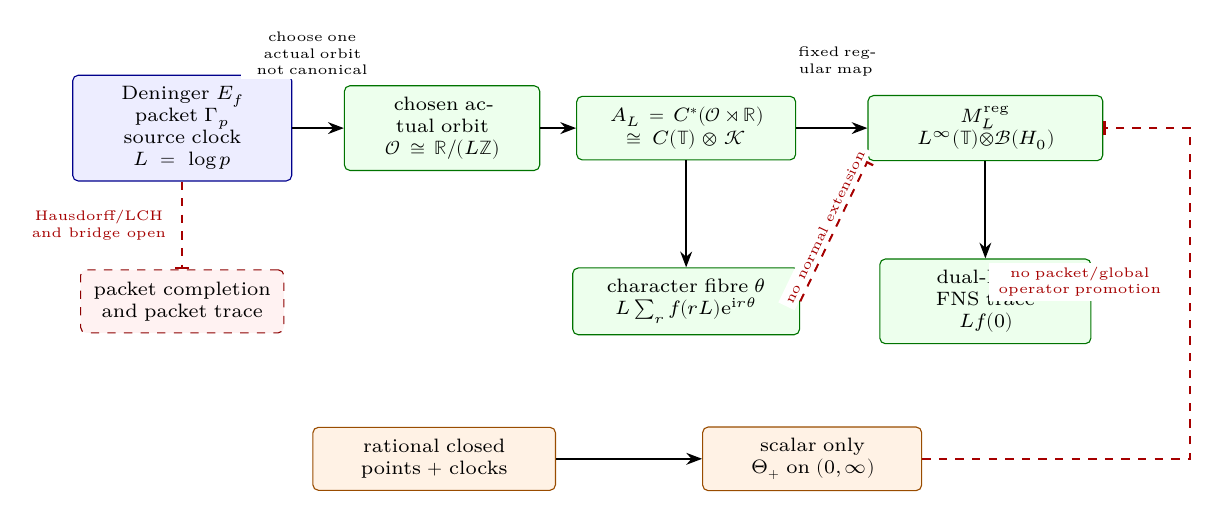
\begin{tikzpicture}[
  x=1cm,y=1cm,
  font=\scriptsize,
  box/.style={draw,rounded corners=2pt,align=center,inner sep=4pt,minimum height=8mm},
  source/.style={box,fill=blue!7,draw=blue!55!black},
  local/.style={box,fill=green!7,draw=green!45!black},
  scalar/.style={box,fill=orange!10,draw=orange!60!black},
  blocked/.style={box,fill=red!5,draw=red!55!black,dashed},
  flow/.style={-{Stealth[length=2mm]},thick},
  stop/.style={-{Bar[width=5pt]},red!65!black,dashed,thick},
  edge label/.style={font=\tiny,fill=white,inner sep=1.5pt,align=center}
]
\node[source,text width=2.5cm] (packet) at (0,2.2)
  {Deninger $E_f$ packet $\Gamma_p$\\source clock $L=\log p$};
\node[local,text width=2.2cm] (orbit) at (3.3,2.2)
  {chosen actual orbit\\$\mathcal O\cong\R/(L\Z)$};
\node[local,text width=2.5cm] (alg) at (6.4,2.2)
  {$A_L=C^*(\mathcal O\rtimes\R)$\\$\cong C(\T)\otimes\K$};
\node[local,text width=2.7cm] (reg) at (10.2,2.2)
  {$M_L^{\mathrm{reg}}$\\$L^\infty(\T)\bar\otimes\B(H_0)$};

\node[blocked,text width=2.3cm] (packetalg) at (0,0)
  {packet completion\\and packet trace};
\node[local,text width=2.6cm] (char) at (6.4,0)
  {character fibre $\theta$\\$L\sum_r f(rL)\e^{\ii r\theta}$};
\node[local,text width=2.4cm] (fns) at (10.2,0)
  {dual-Haar FNS trace\\$Lf(0)$};
\node[scalar,text width=2.8cm] (closed) at (3.2,-2.0)
  {rational closed points $+$ clocks};
\node[scalar,text width=2.5cm] (theta) at (8.0,-2.0)
  {scalar only\\$\Theta_+$ on $(0,\infty)$};

\draw[flow] (packet) -- (orbit);
\node[edge label,text width=1.7cm] at (1.65,3.15)
  {choose one actual orbit\\not canonical};
\draw[flow] (orbit) -- (alg);
\draw[flow] (alg) -- (reg);
\node[edge label,text width=1.7cm] at (8.3,3.05)
  {fixed regular map};
\draw[flow] (alg) -- (char);
\draw[flow] (reg) -- (fns);
\draw[stop] (char.east) -- node[midway,sloped,above,edge label]
  {no normal extension} (reg.south west);
\draw[stop] (packet) -- node[midway,left=4pt,edge label]
  {Hausdorff/LCH\\and bridge open} (packetalg);
\draw[flow] (closed) -- (theta);
\draw[stop] (theta.east) -- ++(3.4,0) -- ++(0,4.2) -- (reg.east);
\node[edge label,text=red!65!black,text width=2.2cm] at (11.4,0.25)
  {no packet/global\\operator promotion};
\end{tikzpicture}

\caption{Typed owner and stop map.  Solid arrows are constructed in this paper or inherited from the cited source; dashed red arrows are unavailable.  The diagram suppresses representation choices and does not assert a packet completion.}\label{fig:owner}
\end{figure}

\section{The locked one-orbit groupoid and its exact completion}

\subsection{Arrow convention, Haar system, and convolution}

Identify \(\mathcal O\) with \(\R/(L\Z)\), written additively, and let \(x\cdot t=x+t\pmod L\).  The transformation groupoid is
\[
 G_L=\mathcal O\rtimes\R=\mathcal O\times\R,
\]
where \((x,t)\) is the arrow from \(x\) to \(x\cdot t\).  Thus
\[
 s(x,t)=x,\quad r(x,t)=x\cdot t,\quad
 (x,t)(x\cdot t,u)=(x,t+u),\quad
 (x,t)^{-1}=(x\cdot t,-t).
\]
Lebesgue measure \(\dd t\) on each source fibre is a continuous Haar system.  On \(C_c(G_L)\) we freeze
\begin{align}
 (F_1*F_2)(x,t)&=\int_{\R} F_1(x,s)F_2(x\cdot s,t-s)\dd s,\label{eq:conv}\\
 F^{*}(x,t)&=\overline{F(x\cdot t,-t)}.\label{eq:star}
\end{align}
The unit space is compact Hausdorff and second countable, so \(G_L\) is LCH and second countable.  Since \(\R\) is amenable, its action is amenable; full and reduced norms coincide \cite[Examples~2.7(2) and Theorem~5.3]{AnantharamanDelaroche2002}.

\subsection{Actual unstabilized completion}

Let \(H=L\Z\subset\R\) be the isotropy subgroup and \(H_0=L^2([0,L),\dd u)\).  Counting measure on \(H\), Lebesgue measure on \(\R\), and quotient length measure \(\dd u\) obey the quotient integral formula
\[
 \int_{\R} g(t)\dd t
 =\int_0^L\sum_{r\in\Z}g(u+rL)\dd u.
\]
This is the specialization of Williams's equation~(4.63) \cite[p.~138]{Williams2007}.

\begin{theorem}[One-orbit groupoid completion]\label{thm:completion}
For the chosen actual orbit,
\[
 A_L:=C^*(G_L)=C_r^*(G_L)
 \cong C^*(L\Z)\otimes\K(H_0)
 \cong C(\T)\otimes\K(H_0).
\]
The isomorphism is actual and unstabilized.  Its displayed continuous-field trivialization depends on the quotient section and compatible induction choices; it is not packet data.
\end{theorem}

\begin{proof}
The action is transitive and \(\mathcal O\cong\R/H\).  Green's theorem gives Morita equivalence with \(C^*(H)\) \cite[Proposition~3, p.~203]{Green1978}, and the transitive groupoid equivalence theorem gives the corresponding compact-operator model \cite[Theorems~2.8 and~3.1]{MuhlyRenaultWilliams1987}.  The stronger statement needed here is Williams's homogeneous-space theorem:
\[
 C_0(\R/H)\rtimes\R
 \cong C^*(H)\otimes\K(L^2(\R/H,\dd u)),
\]
with the quotient measure fixed above \cite[Theorem~4.30, p.~138]{Williams2007}.  It is already unstabilized.  Pontryagin duality identifies \(C^*(L\Z)\) with \(C(\widehat{L\Z})\cong C(\T)\).  Amenability gives the full/reduced equality.  Brown--Green--Rieffel stable isomorphism \cite[Theorem~1.2]{BrownGreenRieffel1977} is consistent with, but is not used to strengthen, the displayed result.
\end{proof}

The algebraic centre of \(C(\T)\otimes\K(H_0)\) is zero because \(H_0\) is infinite-dimensional.  The continuous algebra \(C(\T)\) will reappear in a full finite rank-one corner, not as \(Z(A_L)\).  This distinction is essential in \Cref{sec:corner}.

\subsection{Character convention}

Parametrize \(\widehat H\) by \(\theta\in[0,2\pi)\) and freeze
\begin{equation}
 \chi_\theta(rL)=\e^{\ii r\theta}.\label{eq:character}
\end{equation}
The corresponding induced Hilbert space is realized by quasiperiodic functions satisfying
\begin{equation}
 \eta(u+rL)=\e^{-\ii r\theta}\eta(u),\qquad u\in[0,L),\ r\in\Z.\label{eq:quasi}
\end{equation}
An orthonormal Floquet basis is
\[
 e_{n,\theta}(u)=L^{-1/2}\exp(\ii k_{n,\theta}u),\qquad
 k_{n,\theta}=\frac{2\pi n-\theta}{L}.
\]
The minus sign in \(k_{n,\theta}\) and the plus sign in the eventual return phase are one coupled convention; changing only one is an error.

For \(f\in C_c^\infty(\R)\), let \(a_f\in C_c(G_L)\) be the time kernel \(a_f(x,t)=f(t)\).  We use
\begin{equation}
 \widehat f(\xi)=\int_{\R} f(t)\e^{-\ii t\xi}\dd t.\label{eq:fourier}
\end{equation}
In the induced representation \(\pi_\theta\), translation by \(t\) acts as \(\eta(u)\mapsto\eta(u-t)\), so
\begin{equation}
 \pi_\theta(a_f)e_{n,\theta}
 =\widehat f(k_{n,\theta})e_{n,\theta}.\label{eq:diagonal}
\end{equation}
The compatibility of Green induction with ordinary induced representations is Williams's Theorem~5.12 \cite[p.~161]{Williams2007}; equations \eqref{eq:quasi}--\eqref{eq:diagonal} are its convention-locked specialization.

\section{Character traces and the shifted Poisson formula}

\subsection{Trace class before the trace formula}

Because \(f\in C_c^\infty(\R)\), repeated integration by parts makes \(\widehat f\) rapidly decreasing \cite[Theorems~14.10--14.11, pp.~84--85]{Laugesen2017}.  Hence
\[
 \sum_{n\in\Z}\left|\widehat f\left(\frac{2\pi n-\theta}{L}\right)\right|<\infty
\]
uniformly in \(\theta\).  Thus \(\pi_\theta(a_f)\) is trace class before its trace is taken.  We write
\[
 T_\theta(f):=\Tr(\pi_\theta(a_f)).
\]

\begin{theorem}[Character-fibre Poisson trace]\label{thm:poisson}
For \(f\in C_c^\infty(\R)\) and every \(\theta\in[0,2\pi)\),
\begin{equation}
 T_\theta(f)
 =\sum_{n\in\Z}\widehat f\left(\frac{2\pi n-\theta}{L}\right)
 =L\sum_{r\in\Z}f(rL)\e^{\ii r\theta}.\label{eq:poisson}
\end{equation}
The two series are absolutely convergent.  At \(\theta=0\), every return has coefficient one.
\end{theorem}

\begin{proof}
Apply Poisson summation in the convention \eqref{eq:fourier} \cite[Theorem~23.5, p.~137]{Laugesen2017} to the modulated function \(t\mapsto f(t)\e^{\ii\theta t/L}\), followed by the lattice rescaling \(t\mapsto Lt\).  Its Fourier transform at \(2\pi n/L\) is \(\widehat f((2\pi n-\theta)/L)\), while modulation contributes \(\e^{\ii r\theta}\) at \(t=rL\).  Rapid decay gives absolute convergence and justifies the rearrangement.
\end{proof}

The theorem is local to an already selected orbit.  It does not choose that orbit inside \(\Gamma_p\), supply packet multiplicity, or construct a packet trace.

\subsection[The extended-positive C-star traces]{The extended-positive \(C^*\)-traces}

Fix a compatible induced-character trivialization \(\Phi:A_L\to C(\T)\otimes\K(H_0)\) from \Cref{thm:completion}, satisfying \(\Phi(a)(\theta)=\pi_\theta(a)\).  Evaluation followed by the ordinary compact-operator trace defines
\begin{equation}
 \tau_\theta(a)=\Tr\bigl((\operatorname{ev}_\theta\otimes\operatorname{id})\Phi(a)\bigr),
 \qquad a\in(A_L)_+,\label{eq:taudef}
\end{equation}
with values in \([0,\infty]\).  The trace extends linearly to its trace ideal, which contains every \(a_f\) above.  Pullback of a lower-semicontinuous trace along a \(^{*}\)-homomorphism preserves lower semicontinuity and traciality \cite[Section~3.3 and Theorem~3.11, arXiv-v2 physical p.~12]{ElliottRobertSantiago2011}; trace induction and semifiniteness are consistent with the Morita framework of \cite[Proposition~2.2, pp.~72--73]{CombesZettl1983}.

\begin{proposition}[Character-trace domain]\label{prop:tau}
Each \(\tau_\theta\) is a lower-semicontinuous, densely defined, semifinite, nonfaithful, unbounded \(C^*\)-trace.  On the time-kernel trace ideal,
\[
 \tau_\theta(a_f)=L\sum_{r\in\Z}f(rL)\e^{\ii r\theta},
 \qquad
 \tau_0(a_f)=L\sum_{r\in\Z}f(rL).
\]
\end{proposition}

\begin{proof}
The standard trace on \(\K(H_0)\) is lower semicontinuous, densely defined, and semifinite.  Its pullback through the surjective fibre map has the same first three properties.  Elementary continuous fields with finite-rank compact value form a dense trace-finite ideal.  Nonfaithfulness follows by taking a nonzero positive field \(g\otimes e\) with \(g(\theta)=0\), and unboundedness follows from increasing finite-rank projections in the fibre.  The time-kernel formula is \Cref{thm:poisson}.
\end{proof}

\begin{figure}[htbp]
\centering
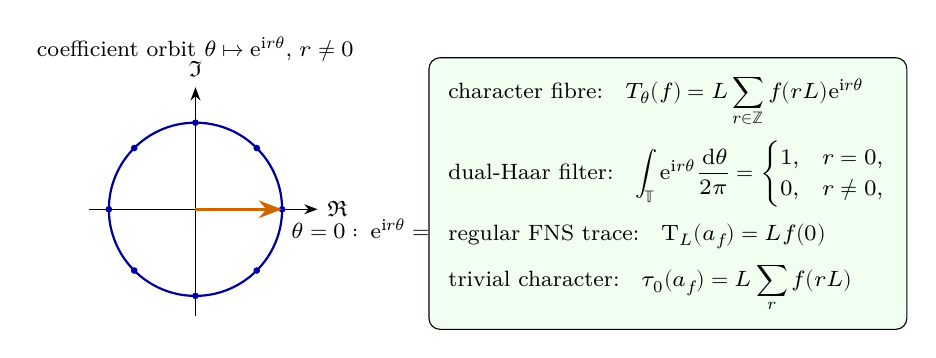
\begin{tikzpicture}[font=\footnotesize,>=Stealth]
  \begin{scope}[xshift=-30mm]
    \draw[->] (-1.35,0) -- (1.55,0) node[right] {$\Re$};
    \draw[->] (0,-1.35) -- (0,1.55) node[above] {$\Im$};
    \draw[thick,blue!60!black] (0,0) circle (1.1);
    \foreach \a in {0,45,...,315}{
      \fill[blue!65!black] ({1.1*cos(\a)},{1.1*sin(\a)}) circle (1.2pt);
    }
    \draw[very thick,orange!80!black,->] (0,0) -- (1.1,0);
    \node[below right] at (1.1,0) {$\theta=0:\;\e^{\ii r\theta}=1$};
    \node[above] at (0,1.75) {coefficient orbit $\theta\mapsto\e^{\ii r\theta}$, $r\ne0$};
  \end{scope}
  \begin{scope}[xshift=30mm,yshift=2mm]
    \node[draw,rounded corners,fill=green!6,align=left,inner sep=7pt] (formula) {
      character fibre:\quad
      $T_\theta(f)=L\displaystyle\sum_{r\in\Z}f(rL)\e^{\ii r\theta}$\\[5pt]
      dual-Haar filter:\quad
      $\displaystyle\int_{\T}\e^{\ii r\theta}\frac{\dd\theta}{2\pi}
       =\begin{cases}1,&r=0,\\0,&r\ne0,\end{cases}$\\[5pt]
      regular FNS trace:\quad $\Tau_L(a_f)=Lf(0)$\\[5pt]
      trivial character:\quad $\tau_0(a_f)=L\displaystyle\sum_r f(rL)$
    };
  \end{scope}
\end{tikzpicture}

\caption{Character coefficient filter.  For every \(r\ne0\), the coefficient \(\e^{\ii r\theta}\) has dual-Haar average zero, whereas its value at the trivial character is one.  The finite-circle picture is explanatory only; the theorem uses Haar integration and absolute summability.}\label{fig:filter}
\end{figure}

\section{The fixed regular trace and exact cancellation}

\subsection{Zak decomposition of the source-fibre representation}

Let \(m\) be normalized dual Haar measure,
\begin{equation}
 \dd m(\theta)=\frac{\dd\theta}{2\pi}.\label{eq:dualhaar}
\end{equation}
This normalization is forced by Fourier isometry for counting Haar on \(L\Z\), in accordance with the uniqueness principle for dual Haar measure and the Plancherel weight \cite[pp.~416--418]{Renault2021}.  It is not the orbit length measure \(\dd u\), nor the orbit probability \(\dd u/L\).

For \(\xi\in C_c(\R)\), define the Zak transform
\begin{equation}
 (Z\xi)(\theta,u)=\sum_{r\in\Z}\xi(u+rL)\e^{\ii r\theta},
 \qquad 0\le u<L.\label{eq:zak}
\end{equation}
Parseval on \(\Z\), followed by the quotient integral formula, gives
\[
 \int_{\T}\int_0^L |Z\xi(\theta,u)|^2\dd u\dd m(\theta)
 =\int_{\R}|\xi(t)|^2\dd t.
\]
Thus \(Z\) extends to a unitary
\[
 L^2(\R)\longrightarrow\int_{\T}^{\oplus} H_0\dd m(\theta).
\]
Moreover \(Z\xi(\theta,u+L)=\e^{-\ii\theta}Z\xi(\theta,u)\), so its fibre is exactly the induced space in \eqref{eq:quasi}.  Direct calculation on \(C_c(G_L)C_c(\R)\) shows that \(Z\) intertwines the source-fibre regular representation \(\lambda_L\) with \(\int_{\T}^{\oplus}\pi_\theta\dd m(\theta)\).

\begin{theorem}[Fixed regular bicommutant and FNS trace]\label{thm:fns}
The source-fibre regular representation is faithful and, under the same Zak trivialization,
\begin{equation}
 M_L^{\mathrm{reg}}:=\lambda_L(A_L)''
 =L^\infty(\T,m)\,\bar\otimes\,\B(H_0).\label{eq:bicommutant}
\end{equation}
The weight
\begin{equation}
 \Tau_L(X)=\int_{\T}\Tr(X(\theta))\dd m(\theta),\qquad X\in(M_L^{\mathrm{reg}})_+,\label{eq:fns}
\end{equation}
is faithful, normal, and semifinite.  For \(f\in C_c^\infty(\R)\), and more generally on the stated bounded \(L^1\) time-kernel domain,
\begin{equation}
 \Tau_L(\lambda_L(a_f))=Lf(0).\label{eq:regular}
\end{equation}
\end{theorem}

\begin{proof}
Faithfulness follows from full/reduced equality and the faithful regular realization.  The Zak unitary makes \(C(\T)\otimes\K(H_0)\) act as continuous compact-operator fields.  Its bicommutant is the decomposable algebra in \eqref{eq:bicommutant}; the model \(vN(\Z)=L^\infty(\T,m)\) and its identity-coefficient trace are standard \cite[pp.~15--16]{Jones2009}.  The tensor product of integration against \(m\) and the ordinary trace is FNS.  On a positive field, Tonelli gives \eqref{eq:fns}; the square-integrable and trace-ideal domains are the usual ones.  On a complex time kernel whose fibre trace norms are integrable, Fubini and \Cref{thm:poisson} give
\begin{align*}
 \Tau_L(\lambda_L(a_f))
 &=\int_{\T} L\sum_{r\in\Z}f(rL)\e^{\ii r\theta}\dd m(\theta)\\
 &=L f(0),
\end{align*}
because \(\int_{\T}\e^{\ii r\theta}\dd m(\theta)=0\) for \(r\ne0\).  The same equality on the bounded \(L^1\) kernel domain follows first on the dense smooth core and then by the trace-norm estimate.
\end{proof}

The construction is the fixed one-orbit analogue of standard invariant-measure traces on continuous crossed products \cite[Proposition~3.2 and Lemma~7.4]{BourneRennie2018}.  It does not identify a packet representation.  Normality of \(\Tau_L\) and full/reduced equality are separate facts.

\begin{table}[htbp]
\centering\small
\caption{Theorem comparison of the two local trace owners.  Both use the length-Haar scale; probability normalization divides the entire trace by \(L\).}\label{tab:traces}
\begin{tabularx}{\textwidth}{P{0.23\textwidth}Y Y}
\toprule
Field & Regular trace \(\Tau_L\) & Character trace \(\tau_\theta\)\\
\midrule
Owner & \(M_L^{\mathrm{reg}}=L^\infty(\T,m)\bar\otimes\B(H_0)\) & \(A_L\cong C(\T)\otimes\K(H_0)\)\\
Type & faithful normal semifinite & l.s.c., densely defined, semifinite, nonfaithful, unbounded \(C^*\)-trace\\
Selection & integrates all characters using \(m=\dd\theta/(2\pi)\) & evaluates one character \(\theta\)\\
Time kernel & \(Lf(0)\) & \(L\sum_r f(rL)\e^{\ii r\theta}\)\\
Nonzero returns & all erased & retained with phase; all have weight one at \(\theta=0\)\\
Completion relation & native FNS owner & no normal extension along the fixed map\\
\bottomrule
\end{tabularx}
\end{table}

\section{The full finite-corner normality obstruction}\label{sec:corner}

\subsection{The same projection in the same represented map}

Choose a rank-one projection \(e\in\K(H_0)\) and set
\[
 q=1_{C(\T)}\otimes e\in A_L.
\]
This projection is full because \(e\) is full in \(\K(H_0)\), and it is trace-finite for every character:
\[
 qA_Lq\cong C(\T),\qquad \tau_\theta(q)=1.
\]
Under the fixed regular embedding \(\iota:A_L\hookrightarrow M_L^{\mathrm{reg}}\), the same projection satisfies
\[
 qM_L^{\mathrm{reg}}q\cong L^\infty(\T,m).
\]
This is a corner statement, not a centre statement.

\begin{theorem}[Fixed-map no-normal-extension]\label{thm:normal}
For every \(\theta\in\T\), there is no normal extended-positive weight \(W\) on \(M_L^{\mathrm{reg}}\) such that
\[
 W(\iota(a))=\tau_\theta(a)\qquad\text{for all }a\in(A_L)_+.
\]
Equivalently, the character trace has no normal extension along this fixed one-orbit regular map.
\end{theorem}

\begin{proof}
Suppose \(W\) exists.  Since \(W(q)=\tau_\theta(q)=1\), compression gives a finite normal positive functional \(\omega(x)=W(qxq)\) on \(qM_L^{\mathrm{reg}}q\cong L^\infty(\T,m)\).  On the continuous corner it agrees with point evaluation at \(\theta\).

Let \(d\) be circular distance and define continuous peaks
\[
 h_n(z)=\max\{1-n d(z,\theta),0\},\qquad n\ge1.
\]
Then \(0\le h_{n+1}\le h_n\le1\), \(h_n(\theta)=1\), and \(h_n\downarrow0\) \(m\)-almost everywhere because singletons have Haar measure zero.  Normality is order continuity on bounded decreasing positive sequences \cite[Definition~7.1.2 and Theorem~7.1.3, pp.~43--44]{Jones2009}, so
\[
 \omega(h_n)\downarrow0.
\]
But agreement with the continuous corner gives \(\omega(h_n)=h_n(\theta)=1\) for every \(n\), a contradiction.
\end{proof}

The theorem refutes only the one-orbit normal-extension analogue.  A packet-level refutation would require a packet algebra, a represented packet map, and a theorem carrying this same projection through restriction, compression, or disintegration.  None is available.

\subsection{What singular extension does mean here}

The phrase ``point evaluation on \(L^\infty\)'' is ill-posed because \(L^\infty\) consists of almost-everywhere equivalence classes.  Nevertheless, the state \(g\mapsto g(\theta)\) on the embedded \(C(\T)\) has state extensions to \(L^\infty(\T,m)\) by positive Hahn--Banach extension.  Every such extension is singular by the peak argument above.

\begin{proposition}[Distinct singular corner states]\label{prop:singular}
There are at least two distinct singular states on \(qM_L^{\mathrm{reg}}q\cong L^\infty(\T,m)\) whose restrictions to \(qA_Lq\cong C(\T)\) are evaluation at \(\theta\).
\end{proposition}

\begin{proof}
Choose a measurable set \(E\) formed from alternating annuli shrinking to \(\theta\), so both \(E\) and \(E^c\) meet every neighbourhood of \(\theta\) in positive Haar measure.  In the measure algebra, the neighbourhood filter of \(\theta\) can be enlarged consistently either by \(E\) or by \(E^c\).  Extend each to an ultrafilter.  The corresponding characters of the abelian \(C^*\)-algebra \(L^\infty(\T,m)\) agree with \(g(\theta)\) for every continuous \(g\), because the ultrafilters converge through all neighbourhoods of \(\theta\), but they take different values on \(1_E\).  Neither character is normal by \Cref{thm:normal}.
\end{proof}

These are extensions only of the finite-corner state.  We construct no singular extended-positive tracial extension of the full unbounded \(\tau_\theta\).

\section{The packet and quotient boundary}

The local proof is now complete, so we can state exactly why it does not decide the primary packet question.  The natural topological action groupoid \(\Gamma_p\rtimes\R\) exists as a set and topological category.  The standard \(C^*\)-completion frozen for this project, however, requires the relevant LCH/Hausdorff hypotheses.  Those hypotheses have not been proved for \(\Gamma_p\).  Replacing it by a product proxy would supply the missing topology by definition and would change the object being tested.

\begin{proposition}[Intrinsic quotient boundary]\label{prop:quotient}
The compact group \(K_p=\R/(L\Z)\) acts continuously and freely on \(\Gamma_p\); the quotient map \(q_p:\Gamma_p\to Q_p\) is open; and \(Q_p\) is quasi-compact and second countable.  For every \(\varphi\in C(\Gamma_p)\),
\begin{equation}
 (\mathcal A_p\varphi)(x)=\frac1L\int_0^L\varphi(x\cdot t)\dd t\label{eq:average}
\end{equation}
is continuous and \(K_p\)-invariant, hence descends to a continuous function on \(Q_p\).  These assertions do not prove that \(Q_p\) is Hausdorff, locally trivial, or equal to a parametrizing base, and \eqref{eq:average} is not a packet Radon-measure or trace theorem.
\end{proposition}

\begin{proof}
Continuity of the residual action follows from the source flow, and freeness follows from exact common isotropy \(L\Z\).  Openness of \(q_p\), quasi-compactness, and second countability were established in Section~2.  Joint continuity of the action and compactness of \(K_p\) imply continuity of the integral in \eqref{eq:average}; Haar invariance makes it constant on orbits.  None of these steps chooses a Borel probability on \(Q_p\) or lifts one through a Radon disintegration.
\end{proof}

Even if a Borel probability on \(Q_p\) were given, the resulting averaging functional would depend on that extra choice for transverse observables.  The source does not select such a probability, prove exhaustion of invariant measures, or choose cross-prime masses.  Packet topology and the packet same-map bridge therefore remain \NOTTESTABLE.  This is the endpoint of the packet branch in this paper.

\section{Scalar ledgers and target-free controls}

\subsection{Local, finite, and positive-time objects}

For a prime \(p\) define the two-sided local scalar return distribution
\begin{equation}
 R_p=L_p\sum_{r\in\Z}\delta_{rL_p},\qquad L_p=\log p.\label{eq:Rp}
\end{equation}
On one chosen orbit, \(R_p(f)=\tau_0(a_f)\).  This equality is only a local trace restriction.  For a finite prime set \(S\), the sum \(R_S=\sum_{p\in S}R_p\) is a finite scalar distribution; it is not a direct-sum operator unless an operator and its domain are separately supplied.

The all-prime object must exclude time zero.  Define
\begin{equation}
 \Theta_+=\sum_{p\ \mathrm{prime}}\log p\sum_{r\ge1}\delta_{r\log p}
 \quad\text{on }(0,\infty).\label{eq:theta+}
\end{equation}

\begin{theorem}[Positive-time scalar ledger]\label{thm:scalar}
The expression \eqref{eq:theta+} defines a positive locally finite Radon measure on \((0,\infty)\).  Its coefficient one is the counting multiplicity of the rational closed point \((p)\), and its factor \(\log p\) is the orbit length.  It is not a packet-orbit multiplicity, a packet trace, or a global \(C^*\)- or \(L^1\)-operator trace.
\end{theorem}

\begin{proof}
Let \(K\subset(0,\infty)\) be compact, with \(K\subset[a,b]\) and \(a>0\).  A term \(r\log p\in K\) implies \(p\le\e^b\), so only finitely many primes occur.  For each such prime, \(1\le r\le b/\log p\), so only finitely many repetitions occur.  Hence \(\Theta_+(K)<\infty\).  Positivity and local finiteness on the locally compact space \((0,\infty)\) give a Radon measure.  The indexing uses the unique rational closed point \((p)\) once; Deninger's clock supplies \(\log p\).  No statement about the number of orbits in \(\Gamma_p\) enters the proof.
\end{proof}

At time zero, summing \(L_p\delta_0\) over all primes has infinite mass.  The positive-time restriction is therefore a mathematical domain condition, not a cosmetic cutoff.

\begin{table}[htbp]
\centering\small
\caption{Theorem-level domain ledger.  Different rows are different typed objects.}\label{tab:domains}
\begin{tabularx}{\textwidth}{P{0.22\textwidth}P{0.25\textwidth}Y Y}
\toprule
Object & Domain & Proved meaning & Forbidden promotion\\
\midrule
\(R_p\) & one prime, all \(r\in\Z\) & scalar distribution; local \(\tau_0(a_f)\) restriction & not a packet trace\\
\(R_S\) & finite \(S\), all \(r\in\Z\) & finite scalar sum & not a global direct-sum operator\\
\(\Theta_+\) & all primes, \(r\ge1\), time \(>0\) & positive locally finite Radon measure & not an all-prime \(C^*/L^1\) trace\\
All-prime two-sided sum & includes \(r=0\) & infinite mass at zero & not defined as a Radon measure on all time\\
\bottomrule
\end{tabularx}
\end{table}

\subsection{Generic clocks and ownership}

The local compiler is not arithmetically unique.  For every \(L>0\), the circle \(\R/(L\Z)\) has the same groupoid completion and the same character/regular trace split.  Composite labels and arbitrary positive clock families also reproduce the analytic formulas.  What distinguishes \eqref{eq:theta+} is source provenance: rational closed points of \(\operatorname{Spec}\Z\) are indexed by primes, not composites, and Deninger's theorem supplies \(L_p=\log p\) before any target comparison.

\begin{proposition}[Generic-clock falsification]\label{prop:generic}
For any locally finite positive clock family \(\{\ell_j\}\) and assigned nonnegative weights \(w_j\), the positive-time expression \(\sum_jw_j\sum_{r\ge1}\delta_{r\ell_j}\) is locally finite under the corresponding properness condition.  Copying a component adds its weight, and composite clocks remain analytically valid.  Therefore local finiteness and the one-orbit character formula alone do not establish arithmetic provenance.
\end{proposition}

The proposition is a falsification boundary: the actual prime record retains arithmetic ownership because its labels and clocks are source-derived; the generic compiler does not grant such ownership to controls.

\subsection{Deterministic controls}

The accompanying standard-library Python suite contains no randomness, network dependency, external dataset, Riemann-zero data, Euler-target comparison, fitted phase, fitted clock, fitted mass, or fitted transverse probability.  The reproduction script ran 18 tests and generated nine CSV artifacts with 129 data rows; two fresh generations were byte-identical.  The locked result-manifest SHA-256 is
\[
 \texttt{20801ebe4c927f939c462842e38569555f96f5fef78859755b6caa8cbcf38b07}.
\]

\begin{table}[htbp]
\centering\small
\caption{Finite target-free controls and their interpretation.  These are regression/falsification witnesses, not theorem proofs.}\label{tab:controls}
\begin{tabularx}{\textwidth}{P{0.29\textwidth}Y Y}
\toprule
Control & What it detects & What it does not establish\\
\midrule
Shifted Poisson and nontrivial phase & coupled minus frequency / plus return-phase convention & infinite Poisson theorem\\
Finite character grid & exact cancellation of represented nonzero modes & Haar-integration theorem\\
Trivial versus regular; zero time & comb versus \(Lf(0)\), with zero exposed & equality or normality of traces\\
Common length/probability scale & both traces rescale together by \(1/L\) & independently fitted normalization\\
Rank-one peaks and representatives & point value survives as Haar mass vanishes; a.e. classes matter & bicommutant or normality proof\\
Transverse probabilities & time-only blindness and transverse-observable variation & a canonical packet probability\\
Copied/arbitrary/composite clocks & additivity and genericity of the compiler & arithmetic provenance\\
Local/finite/positive-time domains & rejects zero-time and all-prime operator conflation & global operator existence\\
\bottomrule
\end{tabularx}
\end{table}

\section{Same-object and Route audit}

\subsection{T0--T7 ownership}

The T0--T7 discipline prevents a proof on one owner from repairing a missing field on another.  T0--T2 record source identity, topology, and clock; T3--T5 record groupoid/Haar, measure, and representation/trace ownership; T6 records the formula and its domain; T7 records arithmetic promotion and coefficient ownership.

\begin{table}[htbp]
\centering\scriptsize
\caption{Status audit for T0--T7 and the five final Route records.  N/A is a type barrier, not a pass.}\label{tab:route}
\begin{tabularx}{\textwidth}{P{0.30\textwidth}Y}
\toprule
Record & Exact \RouteA{} tuple and T0--T7 typed status\\
\midrule
\cand{DEN-EF-PACKET-ACTION-GRPD-P} & \coord{(A0_ANALYTIC_ARITHMETIC_ORIGIN,}\allowbreak\ \coord{A1_WEAK,}\allowbreak\ \coord{A2_FAIL,}\allowbreak\ \coord{A3_FAIL,}\allowbreak\ \coord{A4_FAIL)}\par Actual packet/clock pass partially; packet T1 and T3--T6 are open or \NOTTESTABLE; T7 owns only the prime label and clock.\\
\cand{DEN-EF-ORBIT-ACTION-GRPD} & \coord{(A0_ANALYTIC_ARITHMETIC_ORIGIN,}\allowbreak\ \coord{A1_WEAK,}\allowbreak\ \coord{A2_FAIL,}\allowbreak\ \coord{A3_FAIL,}\allowbreak\ \coord{A4_FAIL)}\par A chosen actual orbit owns local T0--T5 and the local formulas; no packet selection, multiplicity, or cross-prime trace mass.\\
\cand{DEN-EF-ORBIT-GRPD-REG-TRACE} & \coord{(A0_WEAK_ARITHMETIC_RELATION,}\allowbreak\ \coord{A1_FAIL,}\allowbreak\ \coord{A2_FAIL,}\allowbreak\ \coord{A3_FAIL,}\allowbreak\ \coord{A4_FAIL)}\par Fixed FNS owner; T6 is \(Lf(0)\), so nonzero-return A1 is refuted for this trace.\\
\coord{DEN-EF-ORBIT-GRPD-}\newline\coord{TRIVCHAR-TRACE} & \coord{(A0_WEAK_ARITHMETIC_RELATION,}\allowbreak\ \coord{A1_PASS_ANALYTIC,}\allowbreak\ \coord{A2_FAIL,}\allowbreak\ \coord{A3_FAIL,}\allowbreak\ \coord{A4_FAIL)}\par Local l.s.c. trace owns the phase comb and the fixed-map obstruction; no packet mass or normality.\\
\cand{DEN-EF-GRPD-TIME-RETURN-POS} & \coord{(A0_ANALYTIC_ARITHMETIC_ORIGIN,}\allowbreak\ \coord{A1_PASS_ANALYTIC,}\allowbreak\ \coord{A2_FAIL,}\allowbreak\ \coord{A3_FAIL,}\allowbreak\ \coord{A4_FAIL)}\par Scalar type: T3--T5 are N/A, while positive-time T6 and coefficient-one closed-point T7 pass.\\
\bottomrule
\end{tabularx}
\end{table}

Every record has overall verdict 
\texttt{ROUTE\_A\_EXPLORATORY}.  All five have A2, A3, and A4 equal to \texttt{FAIL}; no record owns a determinant, global analytic structure, or natural quantization.  Every final YAML sets \texttt{route\_b\_invocation\_allowed=false}, and there is no \textsc{Route B} record.

The anti-splice rules are immediate from \Cref{tab:route}.  The packet cannot borrow the orbit's LCH completion.  The regular trace cannot borrow the character trace's return comb.  The character trace cannot borrow the regular trace's normality.  The scalar ledger cannot borrow either local operator or a packet completion.  A coordinatewise maximum over these rows would describe no mathematical object.

\section{Limitations and conclusion}

The strongest conclusion is local and negative in a precise sense.  For one already chosen actual Deninger prime orbit, the trivial-isotropy-character trace is a rigorous lower-semicontinuous, densely defined, semifinite, nonfaithful, unbounded \(C^*\)-trace with the entire return comb, but it has no normal extended-positive extension along the fixed Zak-regular map.  The finite corner is full and trace-finite, so the obstruction is not caused by choosing a negligible algebraic ideal.  It is caused by the incompatibility between point-character sensitivity and normality over diffuse dual Haar.

The regular FNS trace is equally rigorous but answers a different question.  It averages the character field and returns \(Lf(0)\).  Its cancellation of every nonzero return is exact, not numerical.  Normality therefore does not coexist with the desired return sensitivity on this fixed local completion.

The primary packet question remains \NOTTESTABLE.  This paper does not prove \(\Gamma_p\) or \(Q_p\) Hausdorff/LCH, a packet groupoid \(C^*\)-completion, a source-selected transverse probability, packet Radon disintegration, packet trace, or a same-map bridge transporting the local corner.  Closing packet Hausdorff/LCH would still leave measure selection and same-map transport as separate problems.  The next smallest topological test is whether the restricted diagonal equivalence relation defining one \(\Gamma_p\) is closed.

The positive-time scalar ledger is a separate \PASS.  It is locally finite because compact positive-time support sees finitely many primes and repetitions, and coefficient one belongs to rational closed-point counting.  It is not evidence that a packet contains one orbit and not an all-prime operator trace.

Finally, the generic-clock controls show why scope matters: the local compiler works for arbitrary and composite clocks.  Arithmetic provenance enters through the source closed points and their \(\log p\) clocks, not through the analytic mechanism alone.  No determinant, A3 or A4 structure, \textsc{Route B}, global spectral operator, or Hilbert--Pólya claim follows.

\appendix

\section{Locked crossed-product convention}

Write \(y-t\) for \(y\cdot(-t)\) on \(\mathcal O\), and set
\[
 \alpha_tg(y)=g(y-t),\qquad F_a(t)(y)=a(y-t,t).
\]
Then \(a\mapsto F_a\) carries the convolution and involution in \eqref{eq:conv} to those of \(C(\mathcal O)\rtimes_\alpha\R\): directly,
\begin{align*}
 (F_a*F_b)(t)(y)&=\int_{\R}a(y-v,v)b(y-t,t-v)\,\dd v=F_{a*b}(t)(y),\\
 F_{a^{*}}(t)(y)&=\overline{a(y,-t)}=\alpha_t(F_a(-t)^{*})(y).
\end{align*}
This is the crossed-product bridge used by the completion and representation arguments, and it is compatible with \eqref{eq:character}--\eqref{eq:diagonal}.  Quotient length Haar has mass \(L\), while orbit probability is \(\dd u/L\).  Passing to probability scale divides both \(\Tau_L\) and every \(\tau_\theta\) by the same \(L\).

\section{Zak Parseval and dense-core identities}

For \(\xi,\zeta\in C_c(\R)\), Fourier orthogonality gives
\begin{align*}
 \int_{\T}\int_0^L (Z\xi)(\theta,u)\overline{(Z\zeta)(\theta,u)}\dd u\dd m(\theta)
 &=\int_0^L\sum_{r\in\Z}\xi(u+rL)\overline{\zeta(u+rL)}\dd u\\
 &=\langle\xi,\zeta\rangle_{L^2(\R)}.
\end{align*}
The compact-support assumption makes the pointwise sums finite; density gives the unitary extension.  Intertwining is checked first for \(F\in C_c(G_L)\) and \(\xi\in C_c(\R)\), where all integrations are absolutely convergent, and then extended by continuity.  In each fibre, \eqref{eq:diagonal} implies
\[
 \|\pi_\theta(a_f)\|_2^2
 =\sum_{n\in\Z}\left|\widehat f\left(\frac{2\pi n-\theta}{L}\right)\right|^2,
\]
and integrating over \(m\) unfolds the shifted intervals to the Fourier Plancherel integral with the locked normalization.

\section{FNS and complex trace domains}

For \(X\in(M_L^{\mathrm{reg}})_+\), \eqref{eq:fns} is defined without assuming finiteness.  Its finite cone is
\[
 \mathfrak M_{\Tau_L}^+=\left\{X\ge0:\int_{\T}\Tr(X(\theta))\dd m(\theta)<\infty\right\}.
\]
The square-integrable left ideal is
\[
 \mathfrak N_{\Tau_L}=\{X:\Tau_L(X^*X)<\infty\},
\]
and the complex trace ideal is the linear span of products \(Y^*X\) with \(X,Y\in\mathfrak N_{\Tau_L}\).  Formula \eqref{eq:regular} for complex \(a_f\) is asserted only after membership in this ideal, supplied by uniform rapid decay for \(C_c^\infty\) kernels.  The bounded \(L^1\) extension means kernels for which the represented field is bounded and the fibre trace norm is \(m\)-integrable; it is not an all-prime \(L^1\) claim.

\section{Lower semicontinuity and projection independence}

For \(a_n\to a\) in norm with all \(a_n,a\ge0\), fibre evaluation is norm continuous and the compact-operator trace is norm lower semicontinuous, hence
\[
 \tau_\theta(a)\le\liminf_n\tau_\theta(a_n).
\]
If \(e_1,e_2\) are rank-one projections in \(\K(H_0)\), a unitary in \(\B(H_0)\) conjugates them.  The resulting corners \(1\otimes e_j\) are Murray--von Neumann equivalent in the multiplier algebra, have character trace one, and yield the same decreasing-peak contradiction.  Thus the obstruction does not depend on a preferred rank-one vector.  Fullness follows because the closed ideal generated by any nonzero rank-one projection in \(\K(H_0)\) is all of \(\K(H_0)\).

\section{Reproduction inventory}

From the repository root, the complete deterministic check is
\begin{center}
\texttt{./papers/8-isotropy-trace/experiments/reproduce.sh}.
\end{center}
It executes 18 unit tests, verifies implementation and active-lock hashes, produces nine CSV artifacts, and compares two fresh generations byte for byte.  The artifacts cover shifted Poisson convention, finite character-grid cancellation, nontrivial character phase, trace scaling, rank-one peaks, \(L^\infty\) representatives, clock/copy/composite controls, transverse-probability controls, and domain boundaries.  The symbolic proofs in the main text remain the theorem owners.

\section{Expanded ownership certificate}

T0 fixes the actual source object; T1 its topology and Borel prerequisites; T2 its flow, clock, and exact isotropy; T3 the groupoid, Haar system, and completion; T4 invariant or transverse measure selection; T5 the represented algebra and trace; T6 the formula with its positive and complex domains; and T7 the arithmetic coefficient and promotion rule.  For the packet, T0 and T2 pass, parts of T1 pass, and T3--T6 are blocked.  For one chosen orbit, T0--T6 close locally, while T7 supplies only the source prime and clock.  For \(\Theta_+\), operator fields T3--T5 are inapplicable by scalar type, whereas T6 and the closed-point-counting part of T7 pass.  These statements reproduce the type barriers in \Cref{tab:route}; they do not create an aggregate candidate.

\section*{Declarations}
\addcontentsline{toc}{section}{Declarations}

\paragraph{Data and code availability.}
No external empirical dataset was used.  Paper~8 uses deterministic Python standard-library code, 18 tests, a reproduction script, nine CSV artifacts, and a hash manifest.  The controls test conventions, falsification cases, and domain regressions; they are not mathematical proofs.  Repository paths and final release hashes are recorded in the accompanying README files.

\paragraph{Ethics approval and consent.}
This work involved no human participants, animals, clinical intervention, or personal data.  Institutional review-board approval, informed consent, and consent for publication are not applicable.

\paragraph{Author contributions.}
Liang Wang: Conceptualization, Methodology, Formal analysis, Investigation, Software, Validation, Data curation, Visualization, Writing---original draft, and Writing---review \& editing.

\paragraph{Competing interests.}
The author declares no financial or non-financial conflict of interest.

\paragraph{Funding.}
No project-specific external funding source was declared.

\paragraph{Generative-AI disclosure.}
Generative AI assisted source triage, proof and domain cross-checking, deterministic-code drafting, adversarial review, manuscript drafting, and formatting.  The workflow retained exact source manifestations, locators, hashes, typed amendments, independent review records, and target-free controls.  No unpublished manuscript was uploaded to a secondary model, and no cross-model review is claimed.  The human author directed the research question and acceptance criteria, must verify every mathematical statement and citation before submission, and takes responsibility for the final manuscript.  An AI system is not an author.

\paragraph{Source and citation integrity.}
All load-bearing sources were retained with versioned manifestations, exact locators, and SHA-256 checksums.  The topology and trace source PDFs, together with the retained novelty corpus, passed the recorded page-count preflights.  For the five groupoid sources, the ARS sidecar preflight was unavailable in the audit environment; their page counts and readable content were instead checked with \texttt{pdfinfo}, text extraction, and representative image fallback.  DOI fields are included only when verified in the source audits.  Technical page locators to Deninger and Morishita refer to the explicitly named arXiv manifestations, not assumed journal pagination.  Redistribution rights for retained PDFs must be checked separately from citation reproducibility.

\paragraph{Acknowledgments.}
No personal acknowledgments are declared.

\bibliographystyle{abbrvnat}
\bibliography{references}

\end{document}
